\chapter{Software Architecture Design}
\label{chap:software-architecture-design}
<TIP: Describe how you design your application using Unified Modelling
Language (UML). There should be at least two diagrams that describe the
software architecture. You may add additional or remove unnecessary diagrams.
However, there needs to be a coherency between them at the end./>

\section{Domain Model}
\label{section:domain-model}
\begin{figure}[h]
    \centering
    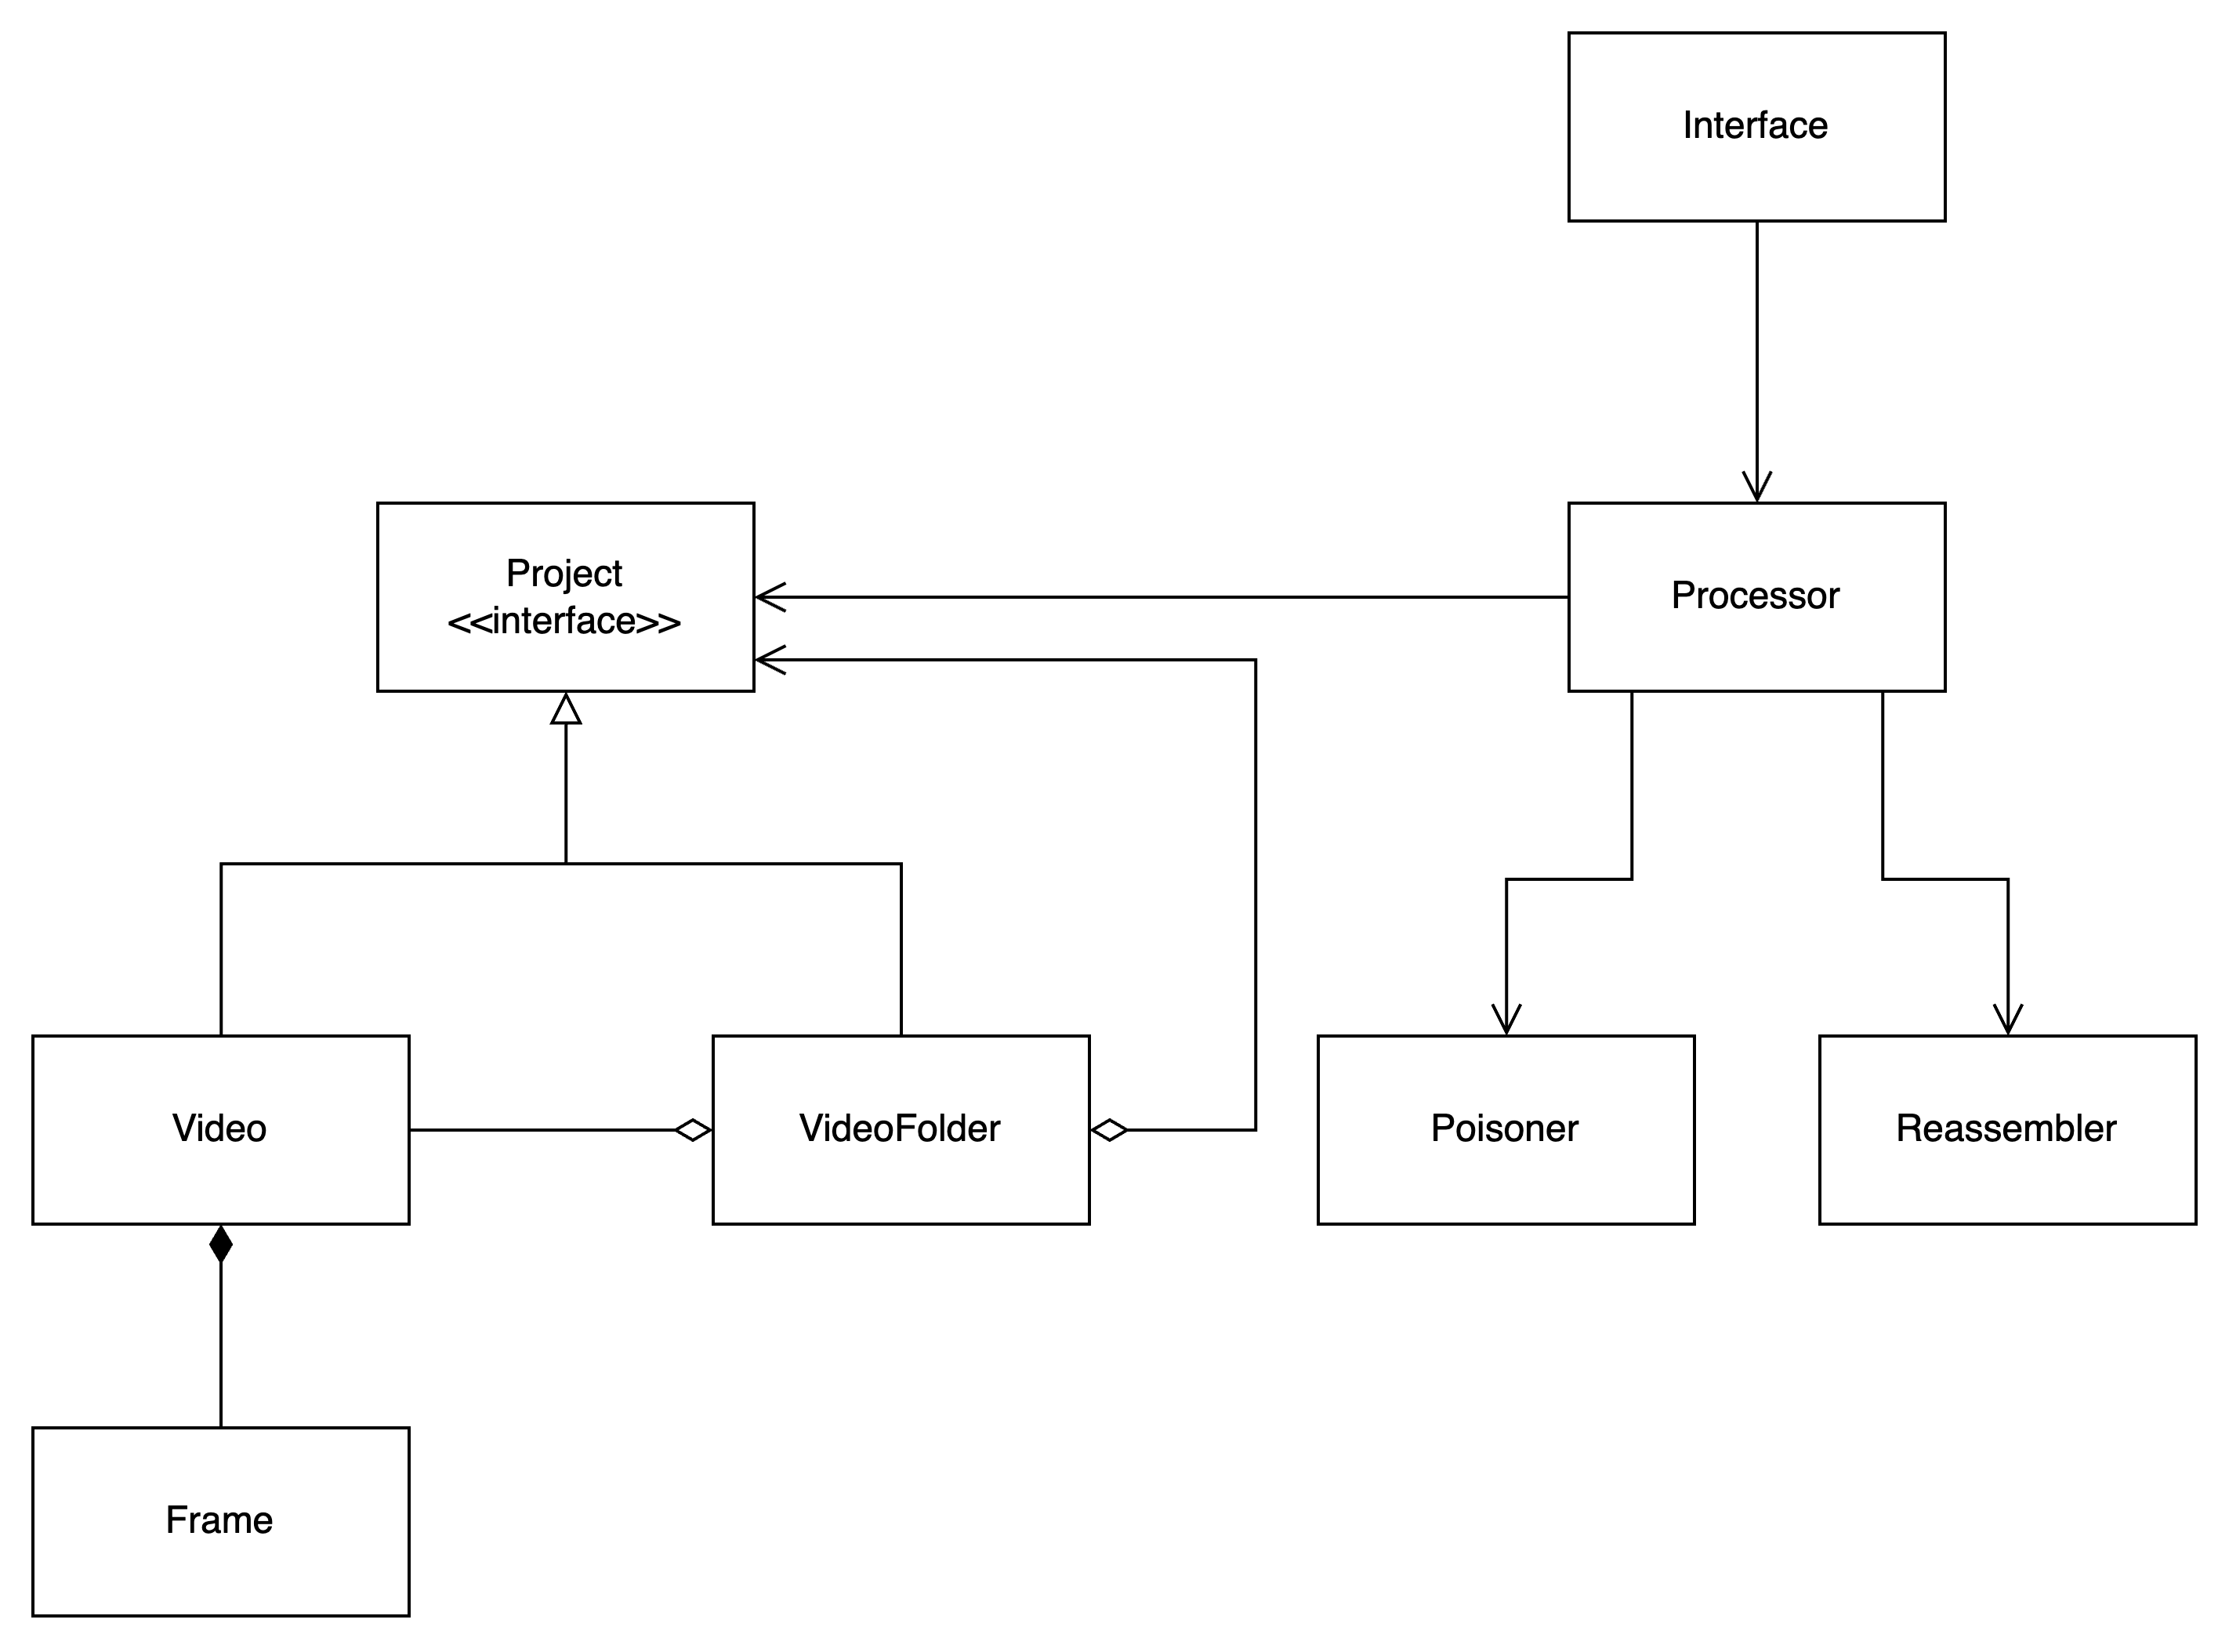
\includegraphics[width=0.8\textwidth]{chapter_4/domain_diagram.png}
    \caption{Domain Diagram}
\end{figure}

\subsection{Interface}
Interface where users interact with the software to input their video and set additional poisoning parameters.

\subsection{Processor}
Processor is a facade controller where it receives video input and output poisened video.

\subsection{Poisoner}
Poisoner manage the process of poisoning frames of the video. Receives frames.

\subsection{Reassembler}
Reassembler manage the process of reassembling videos back into one piece after it has been partitioned to different inferences for parallel computing to optimize poisoning speed.

\subsection{Project}
Project is an interface of the object classes Video and VideoFolder.

\subsection{Video}
Video is an object class containing the necessary information of the video.

\subsection{VideoFolder}
VideoFolder is an object class containing Video objects incase the video needs to be partitioned for parallel computing if the video is long.

\subsection{Frame}
Frame is an object class containing the necessary information of the video frames extracted from the video to send to Poisoner to inject adversarial attack.


\section{Design Class Diagram}
\label{section:design-class-diagram}
<TIP: Showcase a design class diagram for your project and explain
how it works here. You can group classes into packages or layers to communicate your
design better./>

\section{Sequence Diagram}
\label{section:sequence-diagram}
<TIP: Sequence diagrams describe how the software runs at runtime.
You do not have to create a sequence diagram for every scenario. However,
there should be one for all the main ones./>

<ChatGPT: Creating a sequence diagram for every use case is not
strictly necessary, but it can be a valuable tool in certain situations. Sequence
diagrams are particularly useful for illustrating the interactions between different
components or objects in a system over time, showcasing the flow of messages
or actions between them./>